\documentclass[oneside,a4paper,spanish,links,pagenumbers]{amca}
\usepackage{graphicx}
\usepackage{amsmath,amssymb,bm,mathtools}
\usepackage{booktabs,array,tabularx}
\usepackage{microtype}
\usepackage[section]{placeins}
\newcommand{\vect}[1]{\bm{#1}}
\newcommand{\mat}[1]{\bm{#1}}
\newcommand{\skewm}[1]{[\bm{#1}]_{\times}}
\newcommand{\dd}{\mathrm{d}}
\newcommand{\I}{\bm I}
\newcommand{\sym}{\operatorname{sym}}
\newcommand{\diag}{\operatorname{diag}}
\newcommand{\blkdiag}{\operatorname{blkdiag}}
\emergencystretch=2em
\allowdisplaybreaks[1]
\setcounter{tocdepth}{1}
\setcounter{secnumdepth}{3}
\hypersetup{pdftitle={Formulación matemática del modelo estructural y rotodinámico de una turbina eólica},pdfauthor={Nicolás A. Useche Castillo},colorlinks=true,linkcolor=black,citecolor=black,urlcolor=black}
\title{FORMULACIÓN MATEMÁTICA DEL MODELO ESTRUCTURAL Y ROTODINÁMICO DE UNA TURBINA EÓLICA}
\author{Nicolás A. Useche Castillo}
\affil{Departamento de Ingeniería Mecánica, Universidad de los Andes, Bogotá D.C., Colombia}
\begin{document}
\maketitle
\begin{keywords}
Dinámica estructural, viga de Timoshenko, inercia rotacional, sistemas giroscópicos, transformación multiblade.
\end{keywords}
\par
\begin{abstract}
Se desarrolla la formulación matemática de un aerogenerador de eje horizontal constituido por componentes flexibles, masas rígidas y conexiones elásticas. Se especifican las coordenadas, la obtención de las propiedades seccionales y los tensores de inercia, las matrices elementales y el equilibrio con precarga. La contribución giroscópica se obtiene mediante la expansión cuadrática de la energía cinética, incluyendo la rotación de un tensor de inercia anisótropo. Se derivan conjuntamente los términos centrífugos y las transformaciones temporales necesarias para expresar las ecuaciones en ejes inerciales, aplicar restricciones de raíz y obtener coordenadas multiblade. Se completa el planteamiento con cargas externas, problemas de autovalores y excitación sísmica. El documento describe un modelo de pequeñas perturbaciones con inercia evaluada en la configuración nominal y operadores congelados en un azimut; no presenta resultados de simulación ni constituye una formulación aeroelástica no lineal geométricamente exacta.
\end{abstract}
\tableofcontents
\clearpage

\section{PLANTEAMIENTO DEL PROBLEMA}
\label{sec:problema}
Se considera un aerogenerador tripala de eje horizontal, con torre y palas flexibles, una góndola y un cubo representados mediante cuerpos rígidos, y un acoplamiento elástico entre los maestros de góndola y rotor. La velocidad de operación $\Omega$ se prescribe; no se incorpora una ecuación adicional de aceleración del rotor o control del generador. Por consiguiente, una perturbación torsional del tren de potencia no debe identificarse automáticamente con un giro libre de frecuencia nula.

El modelo utiliza vigas de Timoshenko espaciales de dos nodos. La Figura~\ref{fig:modelo} sitúa los componentes. La discretización heredada contiene 138 nodos; los cuatro conectores de penalización se sustituyen por relaciones cinemáticas y permanecen 133 elementos flexibles: 19 de torre, 105 de pala y nueve de transición. Estos últimos conservan las propiedades heredadas y no representan una caracterización independiente de cojinetes.
\begin{figure}[htbp]
\centering
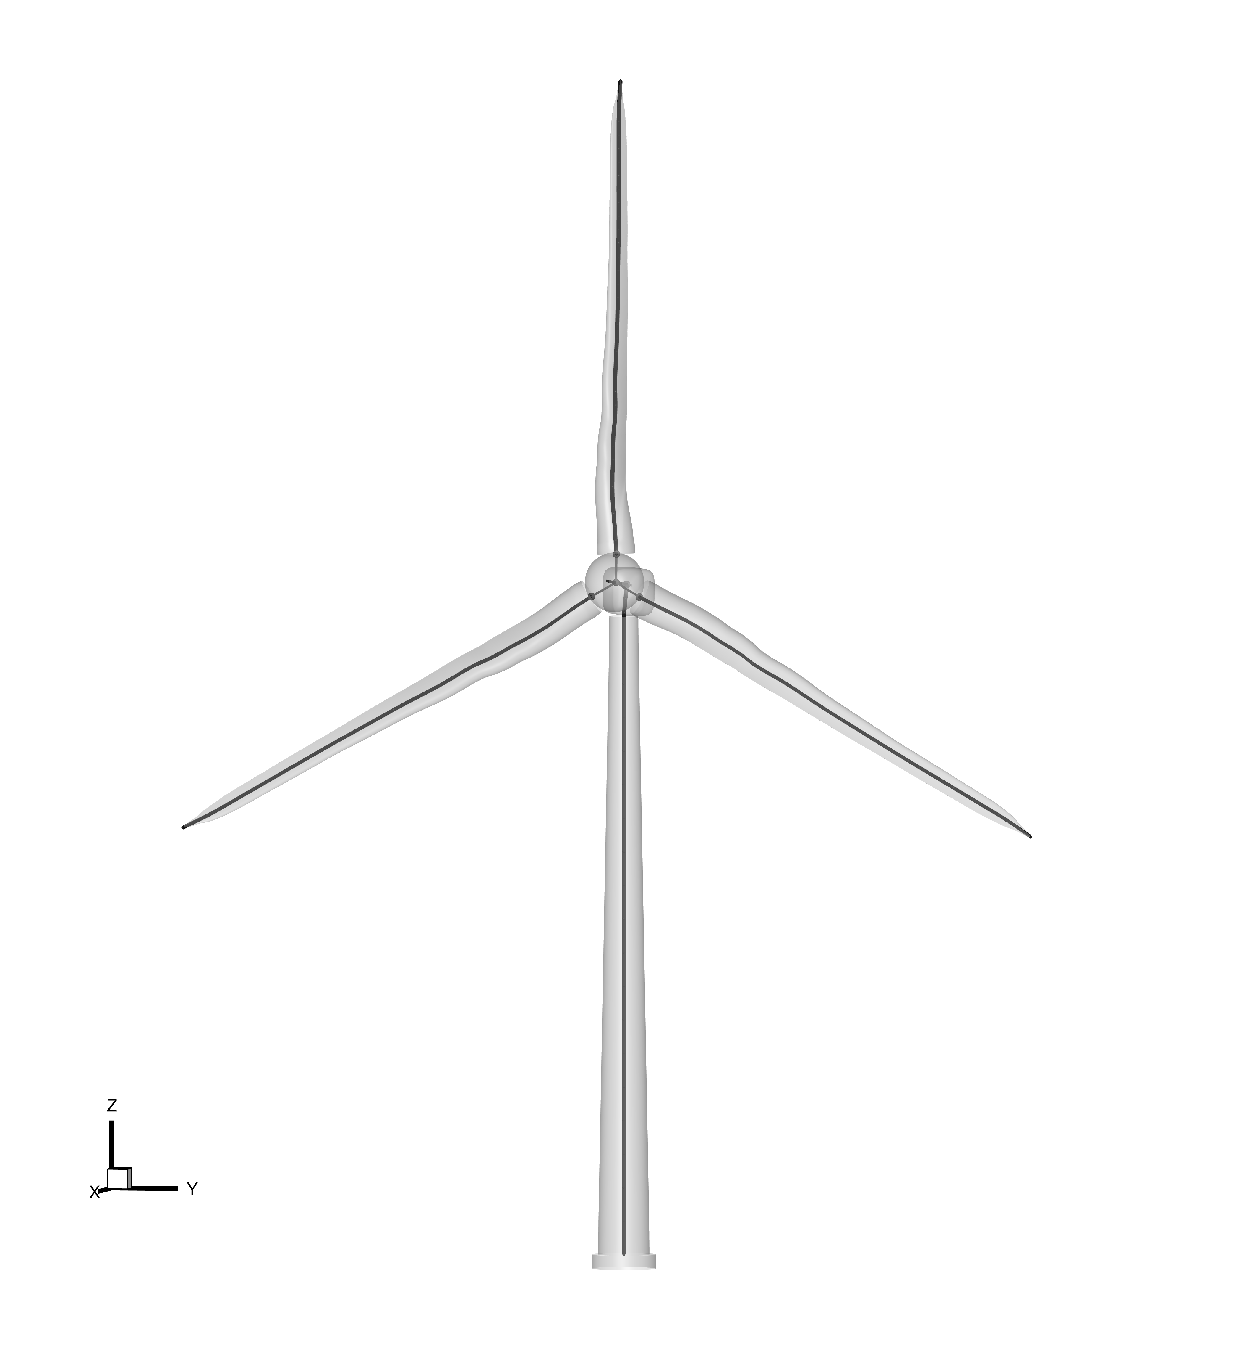
\includegraphics[width=.83\textwidth,height=.42\textheight,keepaspectratio]{modelo.pdf}
\caption{Vista tridimensional del aerogenerador y su idealización estructural. Las líneas y los nodos interiores corresponden a las vigas del modelo existente; las envolventes de torre, palas, góndola y cubo facilitan su identificación. Los perfiles de pala y las carcasas son ilustrativos: no proceden de un modelo CAD ni de una discretización de sólidos. Se conservan las coordenadas nodales y la conectividad del modelo.}\label{fig:modelo}
\end{figure}

Para cada nodo se ordenan las incógnitas como
\begin{equation}
\bm q_i=[u_i,v_i,w_i,\theta_{xi},\theta_{yi},\theta_{zi}]^T.
\end{equation}
La coordenada de equilibrio se denota $\bm q_0$ y la perturbación dinámica $\delta\bm q$. Las masas e inercias se evalúan en la configuración nominal, mientras que la tangente elástica puede incluir la precarga obtenida por equilibrio corrotacional. Esta combinación es una aproximación de inercia de referencia y pequeñas perturbaciones, no una linealización exacta de todas las inercias sobre la geometría deformada.

En coordenadas inerciales de perturbación, la ecuación local en el instante de referencia es
\begin{equation}
\bm M\delta\ddot{\bm q}
+\bigl(\bm C+\bm G_I+\dot{\bm M}\bigr)\delta\dot{\bm q}
+\bm K_I\delta\bm q=\delta\bm f.
\label{eq:global}
\end{equation}
La matriz $\bm G_I$ es antisimétrica; $\dot{\bm M}$ representa transporte de masa, no amortiguamiento material. En coordenadas nominales rotantes con masa constante se recupera la estructura habitual $\bm M\ddot{\bm q}+(\bm C+\bm G_c)\dot{\bm q}+\bm K_c\bm q=\bm f$. La distinción entre ambos sistemas se desarrolla en la sección giroscópica.

\section{COORDENADAS Y PROPIEDADES INERCIALES}
\subsection{Ejes globales y triedro de elemento}
Sea $\{\bm e_X,\bm e_Y,\bm e_Z\}$ el sistema global inercial, con $Z$ vertical. El eje nominal de giro es
\begin{equation}
\bm e_\Omega=\frac{\bm x_{130}-\bm x_{129}}
{\|\bm x_{130}-\bm x_{129}\|},\qquad
\bm\Omega=\Omega\bm e_\Omega,\qquad
\Omega=\frac{2\pi}{60}\,n_{\rm rpm}.
\end{equation}
El origen del marco del rotor se toma en el nodo 130. Para un elemento entre $I$ y $J$, el punto auxiliar $\bm x_a$ define
\begin{align}
L&=\|\bm x_J-\bm x_I\|, &
\bm e_1&=(\bm x_J-\bm x_I)/L,\\
\bm p&=(\I-\bm e_1\bm e_1^T)(\bm x_a-\bm x_I),&
\bm e_3&=\bm p/\|\bm p\|,\qquad \bm e_2=\bm e_3\times\bm e_1.
\end{align}
La matriz $\bm R_e=[\bm e_1,\bm e_2,\bm e_3]^T$ lleva componentes globales a locales. Así,
\begin{equation}
\bm q_e^\ell=\bm T_e\bm q_e^g,
\qquad \bm T_e=\blkdiag(\bm R_e,\bm R_e,\bm R_e,\bm R_e),
\qquad \bm A_e^g=\bm T_e^T\bm A_e^\ell\bm T_e.
\end{equation}
Este cambio geométrico de componentes no sustituye a una transformación temporal de coordenadas.

\subsection{Momentos geométricos y momentos másicos}
Los segundos momentos de área $I_y,I_z$ y la constante torsional $J_t$ tienen dimensión $\mathrm{m^4}$. La masa por longitud $\mu$ y el tensor másico por longitud $\bm j_C$ tienen unidades $\mathrm{kg/m}$ y $\mathrm{kg\,m}$, respectivamente. Para una sección plana en $yz$:
\begin{align}
\mu&=\int_A\rho\,\dd A,&
j_y&=\int_A\rho z^2\,\dd A,&
j_z&=\int_A\rho y^2\,\dd A,\\
j_x&=\int_A\rho(y^2+z^2)\,\dd A=j_y+j_z.
\end{align}
En general, $\bm j_C=\int_A\rho[(\bm r^T\bm r)\I-\bm r\bm r^T]\dd A$; sus términos fuera de diagonal llevan el signo negativo de los productos de coordenadas. La identidad $j_x=j_y+j_z$ no identifica la constante torsional elástica $J_t$ con un momento másico.

Para la torre se adoptan $E=2.10\times10^{11}\ \mathrm{Pa}$, $\nu=0.30$, $G=E/[2(1+\nu)]$ y $\rho_t=7850\ \mathrm{kg/m^3}$. La tabla geométrica suministra $A,A_{sy},A_{sz},J_t,I_y,I_z$, por lo que
\begin{align}
\bm K_s&=\diag(EA,GA_{sy},GA_{sz},GJ_t,EI_y,EI_z),\\
\mu_t&=\rho_t A,\qquad
\bm j_{C,t}=\rho_t\diag(I_y+I_z,I_y,I_z).
\end{align}
Las áreas $A_{sy},A_{sz}$ son efectivas: no se aplica otra corrección cortante.

Las 35 estaciones de pala suministran directamente las seis rigideces generalizadas. Las columnas de masa se interpretan como masa lineal e inercias transversales y se normalizan mediante
\begin{equation}
\begin{gathered}
c_b=\frac{111484}{\displaystyle\sum_{s=1}^{35}
{\rm AXIALD}_s(100/35)},\\
(\mu_s,j_{y,s},j_{z,s})=
c_b({\rm AXIALD}_s,{\rm INERT2}_s,{\rm INERT3}_s).
\end{gathered}
\end{equation}
$c_b$ es un factor adimensional, no una densidad volumétrica. Como la columna polar no aporta una inercia utilizable, se adopta explícitamente $j_{x,s}=j_{y,s}+j_{z,s}$. Los productos seccionales de inercia y los offsets se toman nulos por ausencia de datos. La masa efectiva de una pala se obtiene después como $\sum_e\mu_eL_e$, usando longitudes geométricas reales, sin una segunda renormalización a 100 m.

\subsection{Masa espacial de una sección}
Defínase
\begin{equation}
\bm S(\bm r)=
\begin{bmatrix}0&-r_z&r_y\\r_z&0&-r_x\\-r_y&r_x&0\end{bmatrix},
\quad \bm S(\bm r)\bm a=\bm r\times\bm a,
\quad \bm B_C=[\I,-\bm S(\bm r)].
\end{equation}
Si $\bm r$ une la línea de referencia con el centro de masa, su velocidad incremental es $\bm v_C=\dot{\bm u}-\bm S(\bm r)\dot{\bm\theta}$. De
$T_s=\tfrac12\mu\bm v_C^T\bm v_C+\tfrac12\dot{\bm\theta}^T\bm j_C\dot{\bm\theta}$ se obtiene
\begin{equation}
\boxed{\bm M_s=
\begin{bmatrix}
\mu\I&-\mu\bm S(\bm r)\\
\mu\bm S(\bm r)&\bm j_C-\mu\bm S(\bm r)^2
\end{bmatrix}.}
\label{eq:Ms}
\end{equation}
El término $-\mu\bm S(\bm r)^2=\mu[(\bm r^T\bm r)\I-\bm r\bm r^T]$ es el traslado de Steiner. Los bloques traslacional, acoplado y rotacional de una matriz por longitud tienen unidades distintas: $\mathrm{kg/m}$, $\mathrm{kg}$ y $\mathrm{kg\,m}$.

\subsection{Inercias de góndola y cubo}
Los cuerpos concentrados utilizan masas en kg y tensores en $\mathrm{kg\,m^2}$:
\begin{align}
m_N&=1184500,& \bm J_N^b&=\diag(14806000,32672000,32672000),\\
m_H&=196000,& \bm J_H^b&=2822400\I.
\end{align}
La orientación corporal a global se construye con la convención pasiva ZXZ heredada, convirtiendo grados a radianes. Para $(90^\circ,-5^\circ,-90^\circ)$ resulta
\begin{equation}
\bm Q_b=
\begin{bmatrix}\cos5^\circ&0&\sin5^\circ\\0&1&0\\-\sin5^\circ&0&\cos5^\circ\end{bmatrix},
\qquad \bm J_C^g=\bm Q_b\bm J_C^b\bm Q_b^T,
\qquad \bm r^g=\bm Q_b\bm r^b.
\end{equation}
La rotación conserva los productos de inercia generados: no se diagonaliza de nuevo $\bm J_C^g$. La masa espacial del maestro es
\begin{equation}
\bm M_R=
\begin{bmatrix}
m\I&-m\bm S(\bm r^g)\\
m\bm S(\bm r^g)&\bm J_C^g-m\bm S(\bm r^g)^2
\end{bmatrix}.
\end{equation}
Los offsets de centro de masa de ambos cuerpos se suponen nulos. Esto no elimina los brazos geométricos entre el maestro 130 y las raíces de pala, tratados mediante restricciones cinemáticas.

\section{ELEMENTO ESPACIAL DE TIMOSHENKO}
\subsection{Deformación y energía elástica}
En ejes locales se interpola $\bm\xi(x)=[u,v,w,\theta_x,\theta_y,\theta_z]^T$. Las deformaciones y resultantes conjugadas son
\begin{equation}
\begin{gathered}
\bm\varepsilon=
\begin{bmatrix}u'&v'-\theta_z&w'+\theta_y&\theta_x'&\theta_y'&\theta_z'\end{bmatrix}^T,
\\
\bm n=\begin{bmatrix}N&V_y&V_z&M_x&M_y&M_z\end{bmatrix}^T
=\bm K_s\bm\varepsilon.
\end{gathered}
\end{equation}
Las rotaciones de sección son independientes de las pendientes de la línea media, de modo que se retiene la deformación por cortante. La energía es
\begin{equation}
U_e=\frac12\int_0^L\bm\varepsilon^T\bm K_s\bm\varepsilon\,\dd x,
\qquad \bm K_e^\ell=\int_0^L\bm B^T\bm K_s\bm B\,\dd x.
\end{equation}
Se emplea la interpolación cerrada de dos nodos para secciones desacopladas; la formulación general del método de elementos finitos se encuentra en \citet{reddy2006}.

\subsection{Desglose de la matriz de rigidez}
El vector elemental se ordena como
\begin{equation}
\bm q_e^\ell=[u_I,v_I,w_I,\theta_{xI},\theta_{yI},\theta_{zI},
u_J,v_J,w_J,\theta_{xJ},\theta_{yJ},\theta_{zJ}]^T.
\end{equation}
La matriz $12\times12$ se obtiene insertando cuatro bloques independientes. La extensión ocupa los índices $[1,7]$ y la torsión $[4,10]$:
\begin{equation}
\bm K_a=\frac{EA}{L}\begin{bmatrix}1&-1\\-1&1\end{bmatrix},
\qquad
\bm K_t=\frac{GJ_t}{L}\begin{bmatrix}1&-1\\-1&1\end{bmatrix}.
\end{equation}
Para la flexión en $y$ se utilizan $EI_z$, $GA_y$, los índices $[2,6,8,12]$ y $r=+1$; para la flexión en $z$, $EI_y$, $GA_z$, $[3,5,9,11]$ y $r=-1$. Definiendo
\begin{equation}
\begin{gathered}
\phi=\frac{12EI}{GA_sL^2},\qquad
a=\frac{12EI}{L^3(1+\phi)},\qquad
b=\frac{6EI}{L^2(1+\phi)},\\
c=\frac{(4+\phi)EI}{L(1+\phi)},\qquad
d=\frac{(2-\phi)EI}{L(1+\phi)},
\end{gathered}
\end{equation}
cada bloque de flexión es
\begin{equation}
\boxed{\bm K_b=
\begin{bmatrix}
a&rb&-a&rb\\rb&c&-rb&d\\-a&-rb&a&-rb\\rb&d&-rb&c
\end{bmatrix}.}
\end{equation}
Equivalentemente, si $\bm P_a,\bm P_t,\bm P_y,\bm P_z$ extraen los subconjuntos anteriores,
\begin{equation}
\bm K_e^\ell=\bm P_a^T\bm K_a\bm P_a+\bm P_t^T\bm K_t\bm P_t
+\bm P_y^T\bm K_{by}\bm P_y+\bm P_z^T\bm K_{bz}\bm P_z.
\end{equation}
Esta expresión especifica todas las entradas de la matriz sin omitir los signos cruzados entre desplazamiento y rotación. Cuando $GA_s\to\infty$, $\phi\to0$ y se recupera el límite de Euler--Bernoulli.

\subsection{Interpolación utilizada por la masa y la giroscopía}
Sea $s=x/L$, $\bm p=[1,s,s^2,s^3]$. Para un plano de flexión,
\begin{align}
\bm C_v(\phi)&=\frac{1}{1+\phi}
\begin{bmatrix}
1+\phi&0&0&0\\
-\phi&L(1+\phi/2)&\phi&-L\phi/2\\
-3&-L(2+\phi/2)&3&-L(1-\phi/2)\\
2&L&-2&L
\end{bmatrix},\\
\bm C_r(\phi)&=\frac{1}{1+\phi}
\begin{bmatrix}
0&1+\phi&0&0\\
-6/L&-(4+\phi)&6/L&-(2-\phi)\\
6/L&3&-6/L&3\\0&0&0&0
\end{bmatrix}.
\end{align}
Con $\bm d_y=[v_I,\theta_{zI},v_J,\theta_{zJ}]^T$,
\begin{equation}
v=\bm p\bm C_v(\phi_y)\bm d_y,
\qquad \theta_z=\bm p\bm C_r(\phi_y)\bm d_y,
\qquad \phi_y=\frac{12EI_z}{GA_yL^2}.
\end{equation}
Para $\bm d_z=[w_I,\theta_{yI},w_J,\theta_{yJ}]^T$ se introduce $\bm S_z=\diag(1,-1,1,-1)$:
\begin{equation}
w=\bm p\bm C_v(\phi_z)\bm S_z\bm d_z,
\qquad\theta_y=-\bm p\bm C_r(\phi_z)\bm S_z\bm d_z,
\qquad\phi_z=\frac{12EI_y}{GA_zL^2}.
\end{equation}
Los campos $u$ y $\theta_x$ son lineales entre extremos. Estas seis relaciones definen $\bm\xi=\bm N\bm q_e^\ell$. Derivándolas y formando $v'-\theta_z$ y $w'+\theta_y$ se obtiene $\bm B$.

La masa consistente y el operador giroscópico se integran con la misma cinemática:
\begin{equation}
\bm M_e^\ell=\int_0^L\bm N^T\bm M_s\bm N\,\dd x,
\qquad
\bm G_{c,e}^\ell=\int_0^L\bm N^T\bm G_{c,s}\bm N\,\dd x.
\end{equation}
Para propiedades constantes por elemento, la regla de cuatro puntos de Gauss integra exactamente los productos de grado máximo seis de estas matrices. La misma regla se utiliza para los operadores del potencial centrífugo. La rigidez cerrada se obtiene algebraicamente, no mediante integración reducida.

La variante lineal con integración selectiva utiliza $\bm N=[(1-s)\I_6,s\I_6]$, dos puntos para extensión, torsión y flexión y un punto para los términos que contienen cortante. Admite acoplamientos en $\bm K_s$, pero no es la interpolación cerrada adoptada en el modelo principal.

\section{ENSAMBLAJE, CONEXIONES Y EQUILIBRIO}
\subsection{Ensamblaje y conexiones elásticas}
Si $\bm L_e$ extrae los grados de libertad del elemento, las matrices flexibles se forman por
\begin{equation}
\bm M_{\rm flex}=\sum_e\bm L_e^T\bm M_e^g\bm L_e,
\quad
\bm K_{\rm flex}=\sum_e\bm L_e^T\bm K_e^g\bm L_e,
\quad
\bm M=\bm M_{\rm flex}+\sum_R\bm L_R^T\bm M_R\bm L_R.
\end{equation}
Los maestros 129 y 130 son independientes. Para un brazo $\bm d=\bm x_H-\bm x_N$, la deformación relativa del tren se define mediante
\begin{equation}
\bm\Delta=
\begin{bmatrix}
\bm u_H-\bm u_N+\bm S(\bm d)\bm\theta_N\\
\bm\theta_H-\bm\theta_N
\end{bmatrix}=\bm B_d\bm q,
\quad
\bm K_d=\bm B_d^T\bm k_d\bm B_d,
\quad
\bm C_d=\bm B_d^T\bm c_d\bm B_d.
\end{equation}
El brazo evita rigidez o disipación bajo un movimiento rígido compatible. Una base flexible añade $\bm M_b,\bm C_b,\bm K_b$ a sus coordenadas. Una base fija impone las seis componentes del nodo de cimentación iguales a cero.

\subsection{Energía corrotacional y precarga}
El equilibrio utiliza una energía elemental de pequeñas deformaciones en un marco actualizado. Se calculan la cuerda actual, su longitud $L_c$ y la rotación del marco $\bm\theta_f=\operatorname{axial}\log(\bm Q_c\bm Q_0^T)$. Las rotaciones deformacionales empleadas son
\begin{equation}
\bm\theta_I^d=\bm R_c(\bm\theta_I-\bm\theta_f),
\qquad
\bm\theta_J^d=\bm R_c(\bm\theta_J-\bm\theta_f).
\end{equation}
Con $\bm d_e=[\bm0^T,(\bm\theta_I^d)^T,L_c-L,0,0,(\bm\theta_J^d)^T]^T$,
\begin{equation}
U_e(\bm q_e)=\tfrac12\bm d_e^T\bm K_e^\ell\bm d_e,
\quad \bm f_{{\rm int},e}=\frac{\partial U_e}{\partial\bm q_e},
\quad \bm K_{{\rm int},e}=\frac{\partial^2U_e}{\partial\bm q_e^2}.
\end{equation}
La diferencia de vectores de rotación es una aproximación de pequeñas rotaciones deformacionales; no equivale a componer exactamente rotaciones finitas. El gradiente y la Hessiana se evalúan por diferencias centrales de una misma energía. Para una coordenada $q_i$,
\begin{equation}
f_i\simeq\frac{U(\bm q+h_i\bm e_i)-U(\bm q-h_i\bm e_i)}{2h_i},
\quad
K_{ij}\simeq\frac{U_{++}-U_{+-}-U_{-+}+U_{--}}{4h_ih_j},\quad i\ne j.
\end{equation}
Las entradas diagonales utilizan la segunda diferencia central. La energía axial depende de $L_c-L$; la medida de Green $[(L_c/L)^2-1]/2$ puede recuperarse como descriptor, pero no es la deformación constitutiva que define esta energía.

La ecuación de equilibrio a velocidad prescrita es
\begin{equation}
\bm T_0^T\left[\bm f_{\rm int}(\bm q_0)-\bm f_g
-\bm f_{\rm cf}(\bm q_0)-\bm f_a(\bm q_0,\bm0)-\bm f_{\rm ap}\right]=\bm0,
\qquad \bm q_0=\bm T_0\bm z_0.
\end{equation}
$\bm T_0$ incorpora restricciones y condiciones esenciales en el azimut de referencia. Newton resuelve
\begin{equation}
\bm T_0^T\left(\bm K_{\rm int}-\frac{\partial\bm f_{\rm ext}}{\partial\bm q}\right)
\bm T_0\Delta\bm z
=\bm T_0^T(\bm f_{\rm ext}-\bm f_{\rm int}),
\qquad \bm z_{k+1}=\bm z_k+\alpha_k\Delta\bm z.
\end{equation}
La búsqueda de paso reduce el residual. La continuación en velocidad inicia en $\Omega=0$. El potencial centrífugo de la sección siguiente aporta tanto fuerzas como tangentes: no se añade después una segunda copia de esos términos.

\subsection{Rigidez geométrica por fuerza axial}
Una expresión alternativa de tensión inicial se obtiene de
\begin{equation}
U_g=\frac{N_0}{2}\int_0^L[(v')^2+(w')^2]\,\dd x,
\qquad \bm K_g=N_0\int_0^L\bm N_{\perp}'{}^T\bm N_{\perp}'\,\dd x.
\end{equation}
$N_0>0$ representa tracción. Para un plano de Timoshenko,
\begin{equation}
\bm K_g^{(p)}=\frac{N_0}{(1+\phi)^2}
\begin{bmatrix}
a_g/L&r/10&-a_g/L&r/10\\
r/10&Lc_g&-r/10&-Ld_g\\
-a_g/L&-r/10&a_g/L&-r/10\\
r/10&-Ld_g&-r/10&Lc_g
\end{bmatrix},
\end{equation}
con $a_g=\phi^2+2\phi+6/5$, $c_g=\phi^2/12+\phi/6+2/15$ y $d_g=\phi^2/12+\phi/6+1/30$. Este operador no se suma a la Hessiana corrotacional cuando la precarga ya está incorporada en ella. La matriz geométrica y el ablandamiento por giro tienen orígenes distintos, aunque ambos afecten la rigidez tangente.

\section[GIROSCOPÍA Y TRANSFORMACIONES CINEMÁTICAS]{CINEMÁTICA ROTATORIA, GIROSCOPÍA Y TRANSPORTE ENTRE MARCOS}
\label{prefgyro:section}

Esta sección establece una única cadena cinemática para la masa distribuida de
las palas, el cubo, las restricciones rígidas raíz--cubo y la transformación
multiblade. El punto de partida es una rotación nominal de velocidad angular
constante, impuesta alrededor de un eje conocido, y pequeñas perturbaciones
respecto del equilibrio elástico predeformado. La hipótesis de giro constante es
esencial: no se identifica el movimiento nominal con el de un sólido libre. Si
el eje prescrito no es principal, existe un par de mantenimiento que debe formar
parte de las acciones del punto operativo.

La separación entre movimiento nominal y perturbación sigue la construcción de
pequeñas oscilaciones alrededor de un movimiento estacionario descrita en la
Sección~4.4, ecuaciones (4.51)--(4.70), de \citet{meirovitch1997}. Las matrices
seccionales que se obtienen a continuación son, sin embargo, la especialización
particular adoptada aquí para una sección de viga con traslación, giro y centro
de masa excéntrico; no se atribuyen como una fórmula literal de esa referencia.

\subsection{Energía cinética exacta de una sección}
\label{prefgyro:exacta}

Sea $\bm R_0(t)\in SO(3)$ la orientación nominal del marco que gira con el
rotor y sea

\begin{equation}
 \bm W=[\bm\Omega]_\times,
 \qquad
 \dot{\bm R}_0=\bm R_0\bm W,
 \qquad
 \dot{\bm\Omega}=\bm 0 .
 \label{prefgyro:W}
\end{equation}

Las componentes de $\bm\Omega$ se expresan en el marco nominal. Para una
sección, $\bm a$ es el vector desde el eje de giro hasta el punto de referencia
de la línea de viga, $\bm r$ es el offset desde ese punto hasta el centro de
masa, $m$ es la masa por unidad de longitud y $\bm J$ es el tensor de inercia
centroidal por unidad de longitud. Se introducen la traslación perturbada
$\bm u$ y el vector de rotación perturbada $\bm\theta$ mediante

\begin{equation}
 \bm R(t)=\bm R_0(t)\bm E(\bm\theta),
 \qquad
 \bm E(\bm\theta)=\exp([\bm\theta]_\times).
 \label{prefgyro:Rexacta}
\end{equation}

La posición exacta del centro de masa, salvo una traslación común del origen,
es

\begin{equation}
 \bm x_G=\bm R_0
 \left(\bm a+\bm u+\bm E\bm r\right).
 \label{prefgyro:xG}
\end{equation}

Si $\bm J_\ell(\bm\theta)$ es el Jacobiano izquierdo de $SO(3)$,

\begin{equation}
 \bm J_\ell(\bm\theta)
 =\bm I+\frac{1-\cos\vartheta}{\vartheta^2}[\bm\theta]_\times
 +\frac{\vartheta-\sin\vartheta}{\vartheta^3}
 [\bm\theta]_\times^2,
 \qquad \vartheta=\lVert\bm\theta\rVert,
 \label{prefgyro:Jleft}
\end{equation}

entonces
$\dot{\bm E}\bm E^{\mathsf T}
 =[\bm J_\ell(\bm\theta)\dot{\bm\theta}]_\times$.
Al expresar las velocidades en el marco nominal, donde la rotación
$\bm R_0$ no altera las normas, se obtiene

\begin{align}
 \bm v_G={}&
 \bm W\left(\bm a+\bm u+\bm E\bm r\right)
 +\dot{\bm u}
 +[\bm J_\ell(\bm\theta)\dot{\bm\theta}]_\times
 \bm E\bm r,
 \label{prefgyro:vexacta}\\
 \bm\omega_G={}&
 \bm\Omega+\bm J_\ell(\bm\theta)\dot{\bm\theta}.
 \label{prefgyro:omegaexacta}
\end{align}

La energía cinética exacta por unidad de longitud es, por tanto,

\begin{equation}
 \mathcal T_{\mathrm{exact}}
 =\frac12m\bm v_G^{\mathsf T}\bm v_G
 +\frac12\bm\omega_G^{\mathsf T}
 \bm E\bm J\bm E^{\mathsf T}\bm\omega_G .
 \label{prefgyro:Texacta}
\end{equation}

Esta expresión retiene simultáneamente la velocidad orbital, la velocidad de la
línea de referencia, la excentricidad del centro de masa y la inercia rotacional
anisótropa. En particular, no es correcto añadir a posteriori un bloque de
momento angular a una masa traslacional sin verificar que ambos provienen de la
misma expansión de \eqref{prefgyro:Texacta}.

\subsection{Expansión de segundo orden y matrices seccionales completas}
\label{prefgyro:segundo-orden}

Para obtener las ecuaciones linealizadas se emplean

\begin{align}
 \bm E(\bm\theta)
 & =\bm I+[\bm\theta]_\times
 +\frac12[\bm\theta]_\times^2
 +\mathcal O(\lVert\bm\theta\rVert^3),
 \label{prefgyro:exp2}\\
 \bm J_\ell(\bm\theta)\dot{\bm\theta}
 & =\dot{\bm\theta}
 +\frac12\bm\theta\times\dot{\bm\theta}
 +\mathcal O(3).
 \label{prefgyro:Jleft2}
\end{align}

Resulta útil definir, para dos vectores cualesquiera $\bm a$ y $\bm b$, la
matriz simétrica

\begin{equation}
 \mathcal H(\bm a,\bm b)
 =\frac12\left(\bm a\bm b^{\mathsf T}
 +\bm b\bm a^{\mathsf T}\right)
 -(\bm a^{\mathsf T}\bm b)\bm I,
 \label{prefgyro:Hab}
\end{equation}

que satisface la identidad

\begin{equation}
 \bm a^{\mathsf T}[\bm\theta]_\times^2\bm b
 =\bm\theta^{\mathsf T}\mathcal H(\bm a,\bm b)\bm\theta.
 \label{prefgyro:Hidentity}
\end{equation}

Se agrupan las seis perturbaciones seccionales en
$\bm\eta=[\bm u^{\mathsf T},\bm\theta^{\mathsf T}]^{\mathsf T}$ y se definen

\begin{equation}
 \bm B_G=\begin{bmatrix}\bm I&-[\bm r]_\times\end{bmatrix},
 \quad
 \bm b=\bm a+\bm r,
 \quad
 \bm p=m\bm W\bm b,
 \quad
 \bm h=\bm J\bm\Omega .
 \label{prefgyro:definiciones}
\end{equation}

Aquí $\bm p$ y $\bm h$ son, respectivamente, el momento lineal orbital del
centro de masa y el momento angular centroidal del estado nominal. La parte
cuadrática de la energía puede escribirse como

\begin{equation}
 \mathcal T^{(2)}
 =\frac12\dot{\bm\eta}^{\mathsf T}\bm M_6\dot{\bm\eta}
 +\dot{\bm\eta}^{\mathsf T}\bm A_6\bm\eta
 +\frac12\bm\eta^{\mathsf T}\bm H_\Omega\bm\eta .
 \label{prefgyro:T2}
\end{equation}

La masa seccional completa es

\begin{equation}
 \bm M_6
 =m\bm B_G^{\mathsf T}\bm B_G
 +\begin{bmatrix}\bm 0&\bm 0\\\bm 0&\bm J\end{bmatrix}
 =\begin{bmatrix}
 m\bm I&-m[\bm r]_\times\\
 m[\bm r]_\times&\bm J-m[\bm r]_\times^2
 \end{bmatrix}.
 \label{prefgyro:M6}
\end{equation}

La matriz completa de acoplamiento velocidad--posición es

\begin{equation}
 \bm A_6
 =\begin{bmatrix}
 m\bm W&-m\bm W[\bm r]_\times\\
 m[\bm r]_\times\bm W&
 -m[\bm r]_\times\bm W[\bm r]_\times
 +\mathcal H(\bm p,\bm r)+\bm J\bm W-\tfrac12[\bm h]_\times
 \end{bmatrix}.
 \label{prefgyro:A6}
\end{equation}

El término $\mathcal H(\bm p,\bm r)$ es simétrico y, por consiguiente, no
aparece en la matriz giroscópica. Se conserva para presentar la expansión
completa: con $\bm p,\bm r$ constantes, su contribución es la derivada total
$\frac{\dd}{\dd t}[\tfrac12\bm\theta^{\mathsf T}\mathcal H(\bm p,\bm r)\bm\theta]$
y puede omitirse sin modificar las ecuaciones. La contribución de
velocidad en las ecuaciones de Lagrange es

\begin{equation}
 \boxed{\bm G_6=\bm A_6-\bm A_6^{\mathsf T}}
 =\begin{bmatrix}
 2m\bm W&-2m\bm W[\bm r]_\times\\
 2m[\bm r]_\times\bm W&
 -2m[\bm r]_\times\bm W[\bm r]_\times
 +\bm J\bm W+\bm W\bm J-[\bm h]_\times
 \end{bmatrix}.
 \label{prefgyro:G6}
\end{equation}

Por construcción, $\bm G_6^{\mathsf T}=-\bm G_6$. El bloque rotacional
$\bm J\bm W+\bm W\bm J-[\bm J\bm\Omega]_\times$ es necesario incluso cuando
el centro de masa está sobre la línea de referencia. El bloque reducido
$[\bm J\bm\Omega]_\times$ solo representa una parte asociada al momento
angular nominal: no contiene los términos $\bm J\bm W+\bm W\bm J$ y, por
tanto, no es la expansión completa de \eqref{prefgyro:Texacta}.

La anisotropía muestra la diferencia con claridad. Si $\bm\Omega=\Omega\bm e_1$
y $\bm J=\operatorname{diag}(J_1,J_2,J_3)$ en ejes principales, el acoplamiento
en el plano $2$--$3$ queda multiplicado por

\begin{equation}
 (J_2+J_3-J_1)\Omega,
 \label{prefgyro:principal}
\end{equation}

y no por $J_1\Omega$. Para una inercia no diagonal deben conservarse todos los
productos de inercia de \eqref{prefgyro:G6}.

La Hessiana puramente centrífuga que aparece en \eqref{prefgyro:T2} es

\begin{equation}
 \bm H_\Omega
 =\begin{bmatrix}
 m\bm W^{\mathsf T}\bm W&
 -m\bm W^{\mathsf T}\bm W[\bm r]_\times\\
 m[\bm r]_\times\bm W^{\mathsf T}\bm W&
 -m[\bm r]_\times\bm W^{\mathsf T}\bm W[\bm r]_\times
 +\mathcal H(\bm W^{\mathsf T}\bm p,\bm r)
 +\mathcal H(\bm\Omega,\bm h)
 -\bm W\bm J\bm W
 \end{bmatrix}.
 \label{prefgyro:HOmega}
\end{equation}

La fuerza generalizada constante inducida por el giro se obtiene de la parte
lineal de la energía:

\begin{equation}
 \bm f_{\Omega,0}
 =\bm B_G^{\mathsf T}m\bm W^{\mathsf T}\bm W\bm b
 +\begin{bmatrix}\bm 0\\ \bm h\times\bm\Omega\end{bmatrix}.
 \label{prefgyro:fcentrif}
\end{equation}

Con la convención de almacenar las fuerzas centrífugas en el lado derecho,

\begin{equation}
 \bm f_\Omega(\bm\eta)
 =\bm f_{\Omega,0}+\bm H_\Omega\bm\eta,
 \qquad
 \bm K_{\Omega,c}=-\bm H_\Omega
 \label{prefgyro:KOmega}
\end{equation}

es la contribución correspondiente en el lado izquierdo. Debe sumarse a la
rigidez elástica y a la rigidez geométrica del equilibrio prestresado, no a una
configuración descargada elegida de manera independiente.

Cuando $\bm h$ no es paralelo a $\bm\Omega$, la rotación uniforme prescrita
requiere el par

\begin{equation}
 \bm\tau_{\mathrm{hold}}=\bm\Omega\times\bm h.
 \label{prefgyro:holding}
\end{equation}

Este par se opone al bloque $\bm h\times\bm\Omega$ de
\eqref{prefgyro:fcentrif} y compensa el residuo nominal de Euler. Si no se
aplica, el eje de giro no permanece constante y las hipótesis de
\eqref{prefgyro:W} dejan de ser
válidas. Por ello las ecuaciones anteriores describen un rotor mantenido en su
punto operativo; no constituyen una afirmación sobre la rotación libre de un
sólido anisótropo.

La fuerza centrífuga y el par de mantenimiento participan en el equilibrio de
la turbina completa. Después del ensamblaje, dicho equilibrio tiene la forma

\begin{equation}
 \bm T_0^{\mathsf T}\left[
 \bm f_{\mathrm{int}}(\bm q_0)
 -\bm f_{\mathrm{ext}}^{\mathrm{nc}}(\bm q_0)
 -\bm f_{\Omega}(\bm q_0)\right]=\bm 0,
 \label{prefgyro:equilibrio-nominal}
\end{equation}

donde $\bm f_{\Omega}(\bm q_0)=\bm f_{\Omega,0}+\bm H_\Omega\bm q_0$,
$\bm f_{\mathrm{ext}}^{\mathrm{nc}}$ agrupa las acciones no centrífugas y
$\bm f_{\mathrm{int}}$ incluye las fuerzas elásticas del tren y de la base.
Las reacciones de restricción se eliminan por proyección. No corresponde imponer
$\bm f_{\Omega,0}=\bm 0$ como condición de un rotor libre. Además, la tangente
del par depende de cómo se mantenga la carga durante la perturbación. Con la
convención de residual en el lado izquierdo y coordenadas exponenciales, dos
casos representativos son

\begin{equation}
 \bm K_{\tau}^{\mathrm{cuerpo}}
 =+\frac12[\bm\tau_{\mathrm{hold}}]_\times,
 \qquad
 \bm K_{\tau}^{\mathrm{nominal}}
 =-\frac12[\bm\tau_{\mathrm{hold}}]_\times.
 \label{prefgyro:holding-tangent}
\end{equation}

El primer signo corresponde a componentes constantes en el cuerpo perturbado y
el segundo a componentes constantes en el marco nominal. Si el par proviene de
una ley elástica o de control del tren, debe utilizarse la derivada de esa ley,
en lugar de adoptar uno de estos dos tangentes como regla universal.

Para un elemento de viga, las matrices seccionales se proyectan mediante la
misma interpolación cinemática $\bm N(x)$ usada por la masa consistente:

\begin{equation}
 \bm M_e=\int_0^L\bm N^{\mathsf T}\bm M_6\bm N\,\dd x,
 \quad
 \bm G_{c,e}=\int_0^L\bm N^{\mathsf T}\bm G_6\bm N\,\dd x,
 \quad
 \bm K_{\Omega,c,e}=-\int_0^L
 \bm N^{\mathsf T}\bm H_\Omega\bm N\,\dd x.
 \label{prefgyro:elemento}
\end{equation}

La dependencia de $\bm a(x)$ debe conservarse al evaluar
$\bm f_{\Omega,0}$ y $\bm H_\Omega$. Esta integración común evita combinar una
masa consistente con una giroscopía o una fuerza centrífuga de interpolación
distinta.

\subsection{Transporte de las perturbaciones al marco inercial}
\label{prefgyro:transporte}

Las matrices anteriores están expresadas en componentes corrotantes. Para
acoplar el rotor con la góndola y la torre se transportan todas las
perturbaciones nodales del rotor a ejes inerciales antes de imponer las
restricciones. Sea $\bm q_c=\bm P^{\mathsf T}(t)\bm q_g$ y, en un elemento de
dos nodos,

\begin{equation}
 \bm{\mathcal W}_{12}
 =\operatorname{blkdiag}(\bm W,\bm W,\bm W,\bm W).
 \label{prefgyro:W12}
\end{equation}

Antes de aplicar estas relaciones, las matrices y $\bm W$ se expresan en una misma base de componentes de ensamblaje. En el azimut instantáneo puede elegirse $\bm P=\bm I$ sin perder las derivadas
temporales. Para giro constante,

\begin{equation}
 \dot{\bm q}_c=\dot{\bm q}_g-\bm{\mathcal W}_{12}\bm q_g,
 \qquad
 \ddot{\bm q}_c=\ddot{\bm q}_g
 -2\bm{\mathcal W}_{12}\dot{\bm q}_g
 +\bm{\mathcal W}_{12}^2\bm q_g.
 \label{prefgyro:qtransport}
\end{equation}

Al sustituir \eqref{prefgyro:qtransport} en la ecuación corrotante se obtiene

\begin{align}
 \bm D_g^{\mathrm{in}}&=\bm G_c-2\bm M_e\bm{\mathcal W}_{12},
 \label{prefgyro:Dg-in}\\
 \dot{\bm M}_g&=
 \bm{\mathcal W}_{12}\bm M_e
 -\bm M_e\bm{\mathcal W}_{12},
 \label{prefgyro:Mdot}\\
 \bm G_g&=\bm D_g^{\mathrm{in}}-\dot{\bm M}_g
 =\bm G_c-\bm M_e\bm{\mathcal W}_{12}
 -\bm{\mathcal W}_{12}\bm M_e,
 \label{prefgyro:Gg}\\
 \bm K_{\mathrm{trans}}&=
 -\bm G_c\bm{\mathcal W}_{12}
 +\bm M_e\bm{\mathcal W}_{12}^2.
 \label{prefgyro:Ktransport}
\end{align}

La matriz $\dot{\bm M}_g$ es simétrica y $\bm G_g$ es antisimétrica. En
cambio, el operador total de velocidad

\begin{equation}
 \bm D_g=\bm C_g+\dot{\bm M}_g+\bm G_g
 \label{prefgyro:Dtotal}
\end{equation}

no tiene por qué ser antisimétrico. Exigir antisimetría a $\bm D_g$ eliminaría
precisamente la derivada de la masa producida por una sección anisótropa o por
una interpolación cuya base gira. La rigidez del punto operativo en ejes
inerciales es

\begin{equation}
 \bm K_g^{\mathrm{op}}
 =\bm K_e+\bm K_{\mathrm{prestress}}
 +\bm K_{\Omega,c}+\bm K_{\mathrm{trans}}.
 \label{prefgyro:Koperativa}
\end{equation}

$\bm K_{\mathrm{trans}}$ es un término de transporte de coordenadas y no una
segunda copia de la rigidez centrífuga. Para aceleración angular no nula aparece
además $-\bm M_e\dot{\bm{\mathcal W}}_{12}$ en
\eqref{prefgyro:Ktransport}; dicha extensión queda fuera del punto operativo
de velocidad constante considerado aquí.

Para un cuerpo rígido con centro de masa en el maestro, las mismas identidades
dan, en el bloque rotacional inercial,

\begin{equation}
 \dot{\bm J}_g=\bm W\bm J_g-\bm J_g\bm W,
 \qquad
 \bm D_{\theta,g}=\dot{\bm J}_g-[\bm J_g\bm\Omega]_\times,
 \qquad
 \bm G_{\theta,g}=-[\bm J_g\bm\Omega]_\times.
 \label{prefgyro:rigidbody-inertial}
\end{equation}

Así, una masa cuyo centro coincide con el maestro no recibe un término de
Coriolis traslacional en coordenadas inerciales. El efecto angular del spin
prescrito sí permanece. Para un tensor anisótropo, $\dot{\bm J}_g$ debe
conservarse y el coeficiente completo de velocidad no es puramente
antisimétrico.

\subsection{Restricción raíz--cubo dependiente del tiempo}
\label{prefgyro:mpc}

Las raíces de pala se vinculan al maestro del cubo después del transporte a
componentes inerciales. Si

\begin{equation}
 \bm r_s(t)=\bm R_\Omega(\psi)\bm r_{s0},
 \qquad
 \dot{\bm r}_s=\bm W\bm r_s,
 \qquad
 \ddot{\bm r}_s=\bm W^2\bm r_s,
 \label{prefgyro:rslave}
\end{equation}

la compatibilidad infinitesimal entre maestro $m$ y esclavo $s$ es

\begin{equation}
 \begin{bmatrix}\bm u_s\\\bm\theta_s\end{bmatrix}
 =\bm B_s(t)
 \begin{bmatrix}\bm u_m\\\bm\theta_m\end{bmatrix},
 \qquad
 \bm B_s(t)=
 \begin{bmatrix}
 \bm I&-[\bm r_s(t)]_\times\\
 \bm 0&\bm I
 \end{bmatrix}.
 \label{prefgyro:Bslave}
\end{equation}

Por tanto,

\begin{equation}
 \dot{\bm B}_s=
 \begin{bmatrix}\bm 0&-[\dot{\bm r}_s]_\times\\\bm 0&\bm 0\end{bmatrix},
 \qquad
 \ddot{\bm B}_s=
 \begin{bmatrix}\bm 0&-[\ddot{\bm r}_s]_\times\\\bm 0&\bm 0\end{bmatrix}.
 \label{prefgyro:Bslave-derivadas}
\end{equation}

En las ecuaciones siguientes, el subíndice $f$ denota los operadores completos, anteriores a la reducción de restricciones. Al ensamblar todos los bloques se obtiene
$\bm q_f=\bm T_c(t)\bm q_r$. La reducción dinámica exacta es

\begin{align}
 \bm M_r&=\bm T_c^{\mathsf T}\bm M_f\bm T_c,
 \label{prefgyro:Mred}\\
 \bm D_r&=\bm T_c^{\mathsf T}
 \left(\bm D_f\bm T_c+2\bm M_f\dot{\bm T}_c\right),
 \label{prefgyro:Dred}\\
 \bm K_r&=\bm T_c^{\mathsf T}
 \left(\bm K_f\bm T_c+\bm D_f\dot{\bm T}_c
 +\bm M_f\ddot{\bm T}_c\right).
 \label{prefgyro:Kred}
\end{align}

Una congruencia estática $\bm T_c^{\mathsf T}(\cdot)\bm T_c$ solo es suficiente
cuando $\dot{\bm T}_c=\ddot{\bm T}_c=\bm 0$. La derivada de la masa reducida,

\begin{equation}
 \dot{\bm M}_r
 =\dot{\bm T}_c^{\mathsf T}\bm M_f\bm T_c
 +\bm T_c^{\mathsf T}\dot{\bm M}_f\bm T_c
 +\bm T_c^{\mathsf T}\bm M_f\dot{\bm T}_c,
 \label{prefgyro:Mred-dot}
\end{equation}

permite separar nuevamente la parte simétrica dependiente del tiempo y la
parte giroscópica antisimétrica. Esta construcción mantiene la compatibilidad
en la interfaz sin asignar marcos distintos a la raíz y al cubo.

\subsection{Marco de pala temporal y transformación multiblade}
\label{prefgyro:mbc}

Después de la reducción de las raíces, los grados de libertad flexibles de las
tres palas se expresan en marcos homólogos. Si $\bm Q_{b0}$ contiene como
columnas los ejes locales de la pala $b$ en el azimut de referencia, el cambio
de base local--inercial es

\begin{equation}
 \bm Q_b(\psi)=\bm R_\Omega(\psi)\bm Q_{b0},
 \qquad
 \dot{\bm Q}_b=\bm W\bm Q_b,
 \qquad
 \ddot{\bm Q}_b=\bm W^2\bm Q_b.
 \label{prefgyro:Qblade}
\end{equation}

La matriz $\bm H(\psi)$ se construye colocando
$\operatorname{blkdiag}(\bm Q_b,\bm Q_b)$ en las traslaciones y rotaciones de
cada estación no raíz. En consecuencia,

\begin{equation}
 \dot{\bm H}=\bm{\mathcal W}_H\bm H,
 \qquad
 \ddot{\bm H}=\bm{\mathcal W}_H^2\bm H,
 \label{prefgyro:Htemporal}
\end{equation}

donde $\bm{\mathcal W}_H$ contiene $\bm W$ en los bloques rotantes y ceros en
los grados de libertad estacionarios. Tomar $\dot{\bm H}=\bm 0$ mezclaría una
base local corrotante con perturbaciones declaradas inerciales.

Sea $\bm B_{\mathrm{MBC}}(\psi)$ la transformación armónica colectiva--coseno--
seno para tres palas, con azimuts
$\psi_b=\psi+2\pi(b-1)/3$ \citep{bir2008}. Para un grado de libertad homólogo
por pala, su convención directa y su inversa son

\begin{equation}
 \bm B_{\mathrm{MBC}}=
 \begin{bmatrix}
 1&\cos\psi_1&\sin\psi_1\\
 1&\cos\psi_2&\sin\psi_2\\
 1&\cos\psi_3&\sin\psi_3
 \end{bmatrix},
 \qquad
 \bm B_{\mathrm{MBC}}^{-1}=\frac13
 \begin{bmatrix}
 1&1&1\\
 2\cos\psi_1&2\cos\psi_2&2\cos\psi_3\\
 2\sin\psi_1&2\sin\psi_2&2\sin\psi_3
 \end{bmatrix}.
 \label{prefgyro:Bmbc}
\end{equation}

Con $c_b=\cos\psi_b$, $s_b=\sin\psi_b$ y
$\omega_s=\dot\psi$ constante, las filas de sus derivadas son

\begin{equation}
 [\bm B_{\mathrm{MBC}}]_{b,:}=[1,c_b,s_b],\qquad
 [\dot{\bm B}_{\mathrm{MBC}}]_{b,:}
 =\omega_s[0,-s_b,c_b],\qquad
 [\ddot{\bm B}_{\mathrm{MBC}}]_{b,:}
 =-\omega_s^2[0,c_b,s_b].
 \label{prefgyro:Bmbc-derivadas}
\end{equation}

Para varios grados de libertad homólogos se emplea el producto de Kronecker
con la identidad correspondiente y se conserva la identidad en los grados de
libertad estacionarios. La transformación completa es

\begin{equation}
 \bm P_{\mathrm{MBC}}(\psi)
 =\bm H(\psi)\bm B_{\mathrm{MBC}}(\psi),
 \label{prefgyro:Pmbc}
\end{equation}

y sus derivadas deben conservar ambos orígenes temporales:

\begin{align}
 \dot{\bm P}_{\mathrm{MBC}}
 &=\dot{\bm H}\bm B_{\mathrm{MBC}}
 +\bm H\dot{\bm B}_{\mathrm{MBC}},
 \label{prefgyro:Pdot}\\
 \ddot{\bm P}_{\mathrm{MBC}}
 &=\ddot{\bm H}\bm B_{\mathrm{MBC}}
 +2\dot{\bm H}\dot{\bm B}_{\mathrm{MBC}}
 +\bm H\ddot{\bm B}_{\mathrm{MBC}}.
 \label{prefgyro:Pddot}
\end{align}

Finalmente, para $\bm q_r=\bm P_{\mathrm{MBC}}\bm z$, los operadores en
coordenadas multiblade son

\begin{align}
 \overline{\bm M}
 &=\bm P_{\mathrm{MBC}}^{\mathsf T}
 \bm M_r\bm P_{\mathrm{MBC}},
 \label{prefgyro:Mmbc}\\
 \overline{\bm D}
 &=\bm P_{\mathrm{MBC}}^{\mathsf T}
 \left(\bm D_r\bm P_{\mathrm{MBC}}
 +2\bm M_r\dot{\bm P}_{\mathrm{MBC}}\right),
 \label{prefgyro:Dmbc}\\
 \overline{\bm K}
 &=\bm P_{\mathrm{MBC}}^{\mathsf T}
 \left(\bm K_r\bm P_{\mathrm{MBC}}
 +\bm D_r\dot{\bm P}_{\mathrm{MBC}}
 +\bm M_r\ddot{\bm P}_{\mathrm{MBC}}\right).
 \label{prefgyro:Kmbc}
\end{align}

La coexistencia de $\bm G_g$ con las derivadas MBC no constituye por sí sola un
doble conteo. $\bm G_g$ procede de la energía y del transporte físico de las
perturbaciones, mientras que $\dot{\bm P}_{\mathrm{MBC}}$ y
$\ddot{\bm P}_{\mathrm{MBC}}$ aparecen al reexpresar esas mismas ecuaciones en
coordenadas armónicas. La consistencia exige conservar toda la cadena en el
orden presentado: expansión energética, transporte inercial, restricción
temporal raíz--cubo y, por último, transformación multiblade.


\section{AMORTIGUAMIENTO Y ACCIONES EXTERNAS}
\subsection{Amortiguamiento}
El amortiguamiento mecánico se modela fenomenológicamente sobre las velocidades de perturbación del sistema de ensamblaje:
\begin{equation}
\bm C_s=\alpha\bm M+\beta\bm K_e,
\qquad \zeta_j=\frac{\alpha}{2\omega_j}+\frac{\beta\omega_j}{2}.
\end{equation}
Esta relación para $\zeta_j$ corresponde a los modos del par de referencia $(\bm K_e,\bm M)$ y define los objetivos de calibración de Rayleigh. No representa por sí sola el amortiguamiento modal del problema cuadrático con giro, precarga y términos adicionales.
Dados dos objetivos $(\omega_1,\zeta_1)$ y $(\omega_2,\zeta_2)$,
\begin{equation}
\begin{bmatrix}1/(2\omega_1)&\omega_1/2\\1/(2\omega_2)&\omega_2/2\end{bmatrix}
\begin{bmatrix}\alpha\\\beta\end{bmatrix}
=\begin{bmatrix}\zeta_1\\\zeta_2\end{bmatrix}.
\end{equation}
La rigidez de referencia de Rayleigh es la elástica, no la tangente que contiene términos de transporte. Se suman por separado estructura, cimentación, tren y aerodinámica: $\bm C=\bm C_s+\bm C_b+\bm C_d+\bm C_a$. El término $\dot{\bm M}$ no se incorpora a estos coeficientes de disipación.

\subsection{Gravedad y carga de viento}
La gravedad se introduce consistentemente con la masa:
\begin{equation}
\bm f_{g,e}=\bm M_e^g[\bm g^T,\bm0^T,\bm g^T,\bm0^T]^T,
\qquad
\bm f_{g,R}=\begin{bmatrix}m\bm g\\\bm r_C\times(m\bm g)\end{bmatrix}.
\end{equation}
Para el viento se define una ley general de cargas distribuidas $\bm p_a(x,\bm q,\dot{\bm q},t)$ y momentos $\bm m_a$. Su fuerza elemental equivalente es
\begin{equation}
\bm f_{a,e}=\int_0^L\bm N^T
\begin{bmatrix}\bm p_a\\\bm m_a\end{bmatrix}\dd x,
\qquad \bm f_a=\sum_e\bm L_e^T\bm T_e^T\bm f_{a,e}.
\end{equation}
La ley puede contener dependencia de la velocidad relativa del flujo, de la orientación y de la posición deformada. La formulación no presupone un modelo específico de sustentación, arrastre o inducción. En torno al estado de operación,
\begin{equation}
\delta\bm f_a=\bm F_{a,q}\delta\bm q+\bm F_{a,v}\delta\dot{\bm q}
+\delta\bm f_{a,\rm imp},
\qquad \bm K_a=-\bm F_{a,q},\qquad\bm C_a=-\bm F_{a,v}.
\end{equation}
La misma ley de fuerzas debe definir el equilibrio y sus derivadas. Una carga seguidora puede producir $\bm K_a\ne\bm K_a^T$; no debe imponerse simetría artificial. Cuando no se dispone de derivadas analíticas, cada columna se obtiene por perturbaciones centrales de la coordenada o velocidad correspondiente.

\section{PROBLEMAS MODALES Y MOVIMIENTOS RÍGIDOS}
\subsection{Rotor detenido}
Sin amortiguamiento ni cargas no conservativas, el problema es
\begin{equation}
\bm K\bm\phi_j=\omega_j^2\bm M\bm\phi_j,
\qquad f_j=\omega_j/(2\pi),
\qquad \bm\phi_i^T\bm M\bm\phi_j=\delta_{ij}.
\end{equation}
Un elemento libre de 12 grados de libertad admite seis movimientos rígidos. Para traslación $\bm a$ y giro infinitesimal $\bm b$, el campo nodal
\begin{equation}
\bm u_i=\bm a+\bm b\times\bm x_i,
\qquad \bm\theta_i=\bm b
\end{equation}
produce $\bm\varepsilon=\bm0$ y, por tanto, $\bm K\bm Q_R=\bm0$. Si las seis rigideces seccionales son positivas, el complemento deformacional tiene energía estrictamente positiva; así, $\operatorname{nullity}(\bm K_e)=6$ y $\operatorname{rank}(\bm K_e)=6$. Existen seis frecuencias nulas y seis frecuencias deformacionales positivas. Al empotrar un extremo quedan seis grados de libertad y seis frecuencias positivas.

En un conjunto libre y conectado sin mecanismos internos se conservan seis movimientos rígidos globales. En una base fija no se esperan esos ceros. Su identificación física corresponde al núcleo de la rigidez, no a exigir un exponente decimal particular a la frecuencia calculada. Si $\lambda=\omega^2$ contiene una perturbación numérica de orden $\varepsilon$, la frecuencia asociada puede ser de orden $\sqrt{\varepsilon}$; no es correcto sustituir indiscriminadamente frecuencias pequeñas por cero.

\subsection{Problema cuadrático con giro}
Después de las transformaciones de coordenadas, sean $\widehat{\bm M}$, $\widehat{\bm D}$ y $\widehat{\bm K}$ los operadores en el azimut seleccionado. Con $\bm z=\bm\phi\exp(\lambda t)$:
\begin{equation}
\boxed{\bigl(\lambda^2\widehat{\bm M}
+\lambda\widehat{\bm D}+\widehat{\bm K}\bigr)\bm\phi=\bm0.}
\end{equation}
Una linealización generalizada que evita invertir explícitamente la masa es
\begin{equation}
\begin{bmatrix}\bm0&\I\\-\widehat{\bm K}&-\widehat{\bm D}\end{bmatrix}
\begin{bmatrix}\bm\phi\\\lambda\bm\phi\end{bmatrix}
=\lambda
\begin{bmatrix}\I&\bm0\\\bm0&\widehat{\bm M}\end{bmatrix}
\begin{bmatrix}\bm\phi\\\lambda\bm\phi\end{bmatrix}.
\end{equation}
Para $\lambda=\sigma+\mathrm{i}\omega_d$, se distinguen
\begin{equation}
f_d=\frac{|\omega_d|}{2\pi},\qquad
f_n=\frac{|\lambda|}{2\pi},\qquad
\zeta=-\frac{\sigma}{|\lambda|}.
\end{equation}
Una raíz con $\sigma>0$ representa crecimiento exponencial del sistema congelado. Las propiedades conservativas de \citet[sección 4.7, ecuaciones 4.139--4.148]{meirovitch1997} requieren masa y rigidez simétricas y un término de velocidad puramente antisimétrico; no se trasladan sin comprobación al sistema con aerodinámica, transporte temporal y amortiguamiento.

Las ramas se siguen en velocidad mediante semejanza de formas modales. Para modos recuperados al mismo sistema físico,
\begin{equation}
{\rm MAC}_{ij}=
\frac{|\bm\phi_i^*\bm M_*\bm\psi_j|^2}
{(\bm\phi_i^*\bm M_*\bm\phi_i)(\bm\psi_j^*\bm M_*\bm\psi_j)}.
\end{equation}
$\bm M_*$ es una métrica de masa común. En frecuencias próximas se comparan subespacios, pues una base individual dentro de un subespacio múltiple no es única. Una frecuencia de coordenadas multiblade debe identificarse con su marco; no basta comparar el número de orden de dos autovalores.

\section{EXCITACIÓN SÍSMICA E INTEGRACIÓN TEMPORAL}
En esta sección, $\bm z$ designa las coordenadas independientes anteriores a la transformación multiblade; los operadores llevan el subíndice $r$. El mapa a las coordenadas nodales completas es $\bm T(t)$.
\subsection{Proyección consistente de la aceleración de base}
La aceleración prescrita de base $\bm a_g(t)$ genera
\begin{equation}
\bm f_s^r(t)=-\bm P_g\bm a_g(t),
\qquad \bm P_g=\bm T_0^T\bm M\bm\Gamma_f,
\qquad \bm\Gamma_{\rm eff}=\bm M_r^{-1}\bm P_g.
\end{equation}
$\bm\Gamma_f$ contiene las traslaciones unitarias en las direcciones excitadas, incluidas las coordenadas de apoyo antes de reducir. Esta proyección no se reemplaza, en general, por eliminar filas de una influencia cinemática: la masa consistente conserva acoplamientos con las coordenadas prescritas. Se distingue $\bm\Gamma_{\rm eff}$, que reproduce las fuerzas de inercia, de la influencia cinemática usada para recuperar movimientos absolutos.

La integración actual utiliza $\bm M_r,\bm D_r,\bm K_r$ congeladas en el estado de operación. Por tanto, aproxima la respuesta local del sistema y no integra la evolución periódica completa de geometría, gravedad y restricciones durante muchas revoluciones. Para esta última se necesitarían operadores y mapas actualizados en cada instante.

\subsection{Esquema de Newmark}
Con paso $\Delta t$, el esquema de integración \citep{newmark1971} se escribe
\begin{align}
\bm z_{n+1}&=\bm z_n+\Delta t\dot{\bm z}_n
+\Delta t^2\bigl[(1/2-\beta)\ddot{\bm z}_n+\beta\ddot{\bm z}_{n+1}\bigr],\\
\dot{\bm z}_{n+1}&=\dot{\bm z}_n
+\Delta t\bigl[(1-\gamma)\ddot{\bm z}_n+\gamma\ddot{\bm z}_{n+1}\bigr].
\end{align}
Se adopta aceleración media, $\beta=1/4$ y $\gamma=1/2$. Definiendo $a_0=1/(\beta\Delta t^2)$, $a_1=\gamma/(\beta\Delta t)$, $a_2=1/(\beta\Delta t)$, $a_3=1/(2\beta)-1$, $a_4=\gamma/\beta-1$ y $a_5=\Delta t[\gamma/(2\beta)-1]$:
\begin{align}
\bm K_{\rm eff}&=\bm K_r+a_0\bm M_r+a_1\bm D_r,\\
\bm f_{\rm eff}&=\bm f_{n+1}
+\bm M_r(a_0\bm z_n+a_2\dot{\bm z}_n+a_3\ddot{\bm z}_n)\nonumber\\
&\quad+\bm D_r(a_1\bm z_n+a_4\dot{\bm z}_n+a_5\ddot{\bm z}_n),\\
\bm K_{\rm eff}\bm z_{n+1}&=\bm f_{\rm eff}.
\end{align}
La solución conserva la matriz de velocidad completa, aunque no sea simétrica. Las propiedades del esquema no convierten en estable un sistema físico con raíces de parte real positiva.

\subsection{Recuperación física y reacciones}
Si $\delta\bm q=\bm T(t)\bm z$, las relaciones cinemáticas son
\begin{align}
\delta\dot{\bm q}&=\bm T\dot{\bm z}+\dot{\bm T}\bm z,\\
\delta\ddot{\bm q}&=\bm T\ddot{\bm z}
+2\dot{\bm T}\dot{\bm z}+\ddot{\bm T}\bm z.
\end{align}
Para los operadores congelados se evalúa este mapa y sus derivadas en el mismo azimut de referencia: es una reconstrucción cinemática local, no una trayectoria nominal completa. Las aceleraciones absolutas añaden $\bm\Gamma_f\bm a_g$ a las aceleraciones relativas de perturbación; no incluyen por esa sola operación la aceleración centrípeta nominal del rotor.

El residual completo
\begin{equation}
\bm r=\bm M\delta\ddot{\bm q}
+\bm D\delta\dot{\bm q}+\bm K_I\delta\bm q-\delta\bm f
\end{equation}
contiene reacciones de apoyo y fuerzas de restricción. La proyección $\bm T^T\bm r$ debe satisfacer la ecuación reducida. Las solicitaciones incrementales de viga se recuperan como $\delta\bm n=\bm K_s\bm B\bm T_e\delta\bm q_e$; se suman a las resultantes de precarga cuando se requiere el esfuerzo total.

\section{ALCANCE DE LA FORMULACIÓN}
El planteamiento distingue rigurosamente inercia geométrica y másica, giro prescrito y coordenadas perturbadas, giroscopía y transporte temporal, y rigidez elástica, precarga y potencial centrífugo. La derivación energética determina conjuntamente los términos lineales en velocidad y los cuadráticos en velocidad de giro; su separación no permite omitir los términos que exige un cambio de coordenadas.

Las hipótesis que delimitan el modelo son: secciones equivalentes centradas, inercias de referencia, pequeñas rotaciones deformacionales, velocidad de operación constante y análisis dinámico a azimut congelado. El amortiguamiento, las propiedades del tren, la ley aerodinámica y el movimiento del suelo requieren datos específicos para una predicción física calibrada. La comparación de sistemas giroscópicos debe mantener las mismas coordenadas y la misma ley de excitación. Un análisis periódico completo requeriría un sistema lineal temporal y, para estabilidad, herramientas como Floquet; no se obtiene simplemente promediando operadores de una sola geometría.

\begin{thebibliography}{9}
\bibitem[Meirovitch(1997)]{meirovitch1997}
Meirovitch, L. \emph{Principles and Techniques of Vibrations}. Prentice Hall, 1997. Secciones 4.4, 4.7 y 7.17; ecuaciones de pequeñas oscilaciones alrededor del movimiento estacionario: (4.51)--(4.70).
\bibitem[Reddy(2006)]{reddy2006}
Reddy, J.N. \emph{An Introduction to the Finite Element Method}. 3.\textsuperscript{a} edición, McGraw-Hill, 2006.
\bibitem[Bir(2008)]{bir2008}
Bir, G.S. \emph{Multi-Blade Coordinate Transformation and Its Application to Wind Turbine Analysis}. NREL/CP-500-42553, 2008.
\bibitem[Newmark y Rosenblueth(1971)]{newmark1971}
Newmark, N.M. y Rosenblueth, E. \emph{Fundamentals of Earthquake Engineering}. Prentice Hall, 1971.
\end{thebibliography}
\end{document}
